%---------------------------------------------------------------------------
% Content of Chapter 5 - System architecture
%
%---------------------------------------------------------------------------


\chapter{System architecture}
\label{cha:sys_arch}


\section{Introduction}
\label{sec:gui}

Design stage is probably most important in whole application life cycle. Decisions made during this step affects 
all following stages. Properly designed architecture of system or application reduces possibility of pitfalls during
implementation stage. It also allows easier extension, growth of application, as well as better integration with other
systems, thus extends application's lifetime. 

While designing application I have been trying to follow few well known, software design principles, like:
\begin{itemize}
 \item {\bf Single Responsibility
principle}~~~~~~~~~~~~~~~~~~~~~~~~~~~~~~~~~~~~~~~~~~~~~~~~~~~~~~~~\linebreak
Application should be divided into distinct features with as
little overlap as possible. Architecture should strain to minimize amount of interaction points to achieve high cohesion
and low coupling.
 \item {\bf Principle of Least Knowledge (Law of Demeter~-~LoD)}~~~~~~~~~~~~~~~~~~~~~~~~~~~~~~~~~~~~~~~~~\linebreak
Each component or module should be responsible for only a specific feature or functionality, or aggregation of cohesive
functionality.
 \item {\bf Don't repeat yourself (DRY)}~~~~~~~~~~~~~~~~~~~~~~~~~~~~~~~~~~~~~~~~~~~~~~~~~~~~~~~~\linebreak
You should only need to specify intent in one place. For example, in terms of application design, specific functionality
should be implemented in only one component; the functionality should not be duplicated in any other component.
 \item {\bf Keep It Simple Stupid! (KISS)}~~~~~~~~~~~~~~~~~~~~~~~~~~~~~~~~~~~~~~~~~~~~~~~~~~~~~~~~\linebreak
It's a broad principle, but works in software architecture domain quite well. Generally speaking, it states that while
designing application, one should try to avoid creating unnecessarily complex structures.
\end{itemize}

In this chapter, I would like to describe architecture of proposed system. First, in Section~\ref{sec:decomposition} I
will try to distinguish high level components, describe them roughly and present most important data flows between
components. Following subsequent sections
(\ref{sec:arch_gui},~\ref{sec:arch_monitoring_hub},~\ref{sec:arch_monitoring_hub_application}
,~\ref{sec:arch_knowledge}, and~\ref{sec:arch_tproxy}) contains deeper analysis of each high level component, which
constitutes good base for further development


%---------------------------------------------------------------------------


%---------------------------------------------------------------------------
% System Decomposition.
%
%---------------------------------------------------------------------------


\section{Decomposition}
\label{sec:arch_decomposition}

During design stage several high level components have been introduced. All distinguished components, with
relationships between them can be found in Figure~\ref{fig:arch_overall}. What also should be noticed is that
only highest level components are covered in this section. Each of those components should be interpreted as
independent component that is either standalone application or library, with API containing one or more
interfaces. This API is then shared between provider, which is component that realizes given interface and consumer -
module that actually uses those functionalities to realize its own aims.
Following subsection tries to depict those components and describe them roughly. 

\begin{figure}[ht]
  \centering
  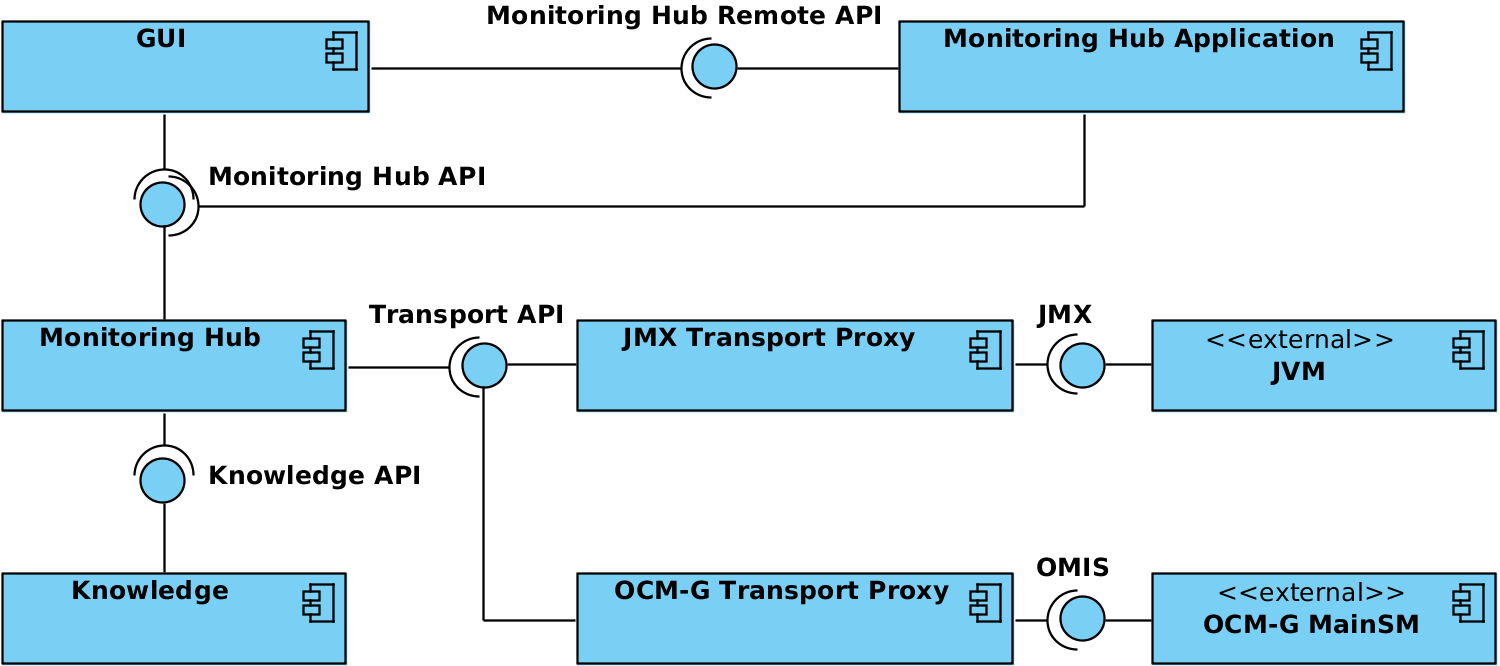
\includegraphics[width=1\textwidth]{arch_overall}
  \caption{Overall system decomposition}
  \label{fig:arch_overall}
\end{figure}

\subsection{Components overview}
 
As can be seen in Figure~\ref{fig:arch_overall}, system has been decomposed into 8 high-level components. Those are:

\begin{itemize}
 \item {\bf GUI}~~~~~~~~~~~~~~~~~~~~~~~~~~~~~~~~~~~~~~~~~~~~~~~~~~~~~~~~\linebreak
Graphic User Interface. GUI is standalone, desktop application, used by user directly. Provides to him facilities
allowing management of whole system. Doesn't perform any measurements or analysis, it only gives control over other
components (direct or indirect) and visualizes results of measurements.

GUI application contains embedded Monitoring Hub, which allows system to operate also in smallest scale - single
measuring process with one or more measured processes attached to it directly. Additionally it connects to
Monitoring Hub Application which allows using Monitoring Hub remotely.

 \item {\bf Monitoring Hub}~~~~~~~~~~~~~~~~~~~~~~~~~~~~~~~~~~~~~~~~~~~~~~~~~~~~~~~~\linebreak
Most important component. Contains all logic needed for resources and measurements management. To fulfill it's
duties it uses Knowledge and Transport Proxies (one or more implementation) components. At this stage of development
only JMX and OCM-G transport proxies will be provided, but proposed architecture allows ease addition of new proxies. 

Monitoring Hub doesn't work as standalone application. Instead, it is in form of library (Java jar) that will be used by
other components that will work as processes. Monitoring Hub component is used by GUI (in embedded mode) and by
Monitoring Hub Application.

 \item {\bf Monitoring Hub Application}~~~~~~~~~~~~~~~~~~~~~~~~~~~~~~~~~~~~~~~~~~~~~~~~~~~~~~~~\linebreak
Standalone, command line application (or daemon if possible) that exposes services of Monitoring Hub to other
components with remote access through the network (either LAN or WAN). It can accept remote connections from GUI
components.

It's main responsibility is to allow system to work in distributed manner. Having process that is separate, and
independent from GUI application, which continuously measures work of long lasting jobs is crucial to allow measuring
system to scale up. 

 \item {\bf Knowledge}~~~~~~~~~~~~~~~~~~~~~~~~~~~~~~~~~~~~~~~~~~~~~~~~~~~~~~~~\linebreak
Knowledge component is realizes semantic approach of application. It provides ontology functionalities to
Monitoring Hub. It's responsible for initializing ontology database and response to all queries issued by Monitoring Hub
regarding relationships between resource types, resources or capabilities.

This component is in form of a library that is dependency for Monitoring Hub, and must be included in both GUI and
Monitoring Hub Application distributions.


 \item {\bf JMX Transport Proxy}~~~~~~~~~~~~~~~~~~~~~~~~~~~~~~~~~~~~~~~~~~~~~~~~~~~~~~~~\linebreak
Transport proxy component, which can communicate with JVM processes using JMX protocol. It's main responsibilities
include: establishing connection with JVM, mapping between generic, knowledge-based resources or capability value
requests into Java specific components or JMX queries.

 \item {\bf OCM-G Transport Proxy}~~~~~~~~~~~~~~~~~~~~~~~~~~~~~~~~~~~~~~~~~~~~~~~~~~~~~~~~\linebreak
Transport proxy component, which communicates with OCM-G MainSM monitor. It allows integration with visualization of
measurements performed by OCM-G applications monitored. It's responsibility is similar to the one of JMX Transport Proxy
- establish and maintain connection to MainSM, translate queries given in ontology terms to OMIS specific requests.

\end{itemize}


\subsection{Interfaces overview}

To decouple all proposed components, system will be using following interfaces:

\begin{itemize}
 \item {\bf Monitoring Hub API}~~~~~~~~~~~~~~~~~~~~~~~~~~~~~~~~~~~~~~~~~~~~~~~~~~~~~~~~\linebreak
Interface for core system's logic. Describes methods for managing every aspect of system - measurements, visualizations
and resources management. It is realized by Monitoring Hub component and used by GUI. 

 \item {\bf Monitoring Hub Remote API}~~~~~~~~~~~~~~~~~~~~~~~~~~~~~~~~~~~~~~~~~~~~~~~~~~~~~~~~\linebreak
This interface is a derivative of Monitoring Hub API. It contains same set of functionalities, with addition
of operations specific to remote access. This includes: registration of remote listener, remote
interface wrapper for Monitoring Hub allowing passing remote exceptions.

 \item {\bf Transport API}~~~~~~~~~~~~~~~~~~~~~~~~~~~~~~~~~~~~~~~~~~~~~~~~~~~~~~~~\linebreak
Common interface for communication with data access services. Currently realized by all JMX and OCM-G Transport Proxy
component. To add support of other data sources in future - this interface will have to be implemented.

 \item {\bf Knowledge API}~~~~~~~~~~~~~~~~~~~~~~~~~~~~~~~~~~~~~~~~~~~~~~~~~~~~~~~~\linebreak
Interface describing operations related to ontology maintenance and usage. Realized by Knowledge component, used
by Monitoring Hub. 
\end{itemize}



\subsection{Most important data flows}

\begin{figure}[ht]
  \centering
  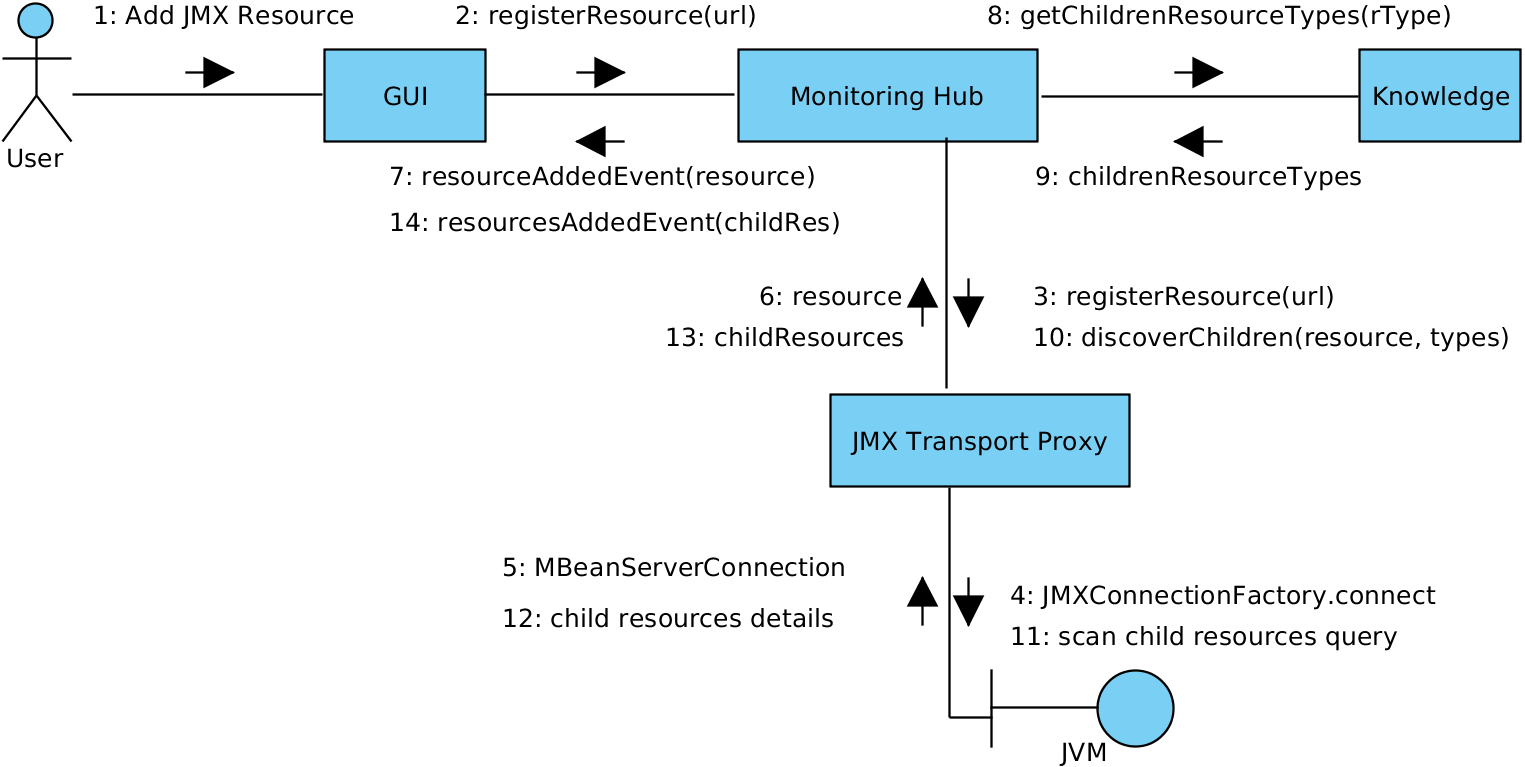
\includegraphics[width=0.9\textwidth]{comm_add_resource}
  \caption{Communication diagram - adding of new resource}
  \label{fig:comm_add_resource}
\end{figure}

Figure~\ref{fig:comm_add_resource} contains communication diagram covering adding new resource action. This action is
initialized by User actor. User starts flow by performing actions (like button click or wizard - not covered here) on
GUI component. In response to this event, GUI sends request to Monitoring Hub, asking to register new resource,
using parameters provided by the user. In subsequent step, Monitoring Hub first lookups in it's dictionary of all
registered transport proxies, the one that can communicate with resource specified by user. After finding valid
transport proxy, Monitoring Hub passes the registration request to it. In this case, JMX
Transport Proxy tries to initialize connection to JVM using URL provided by user in first step. After successful
connection, JVM creates and initializes Resource object. This includes gathering basic attributes describing object
as well as setting all meta data that proxy will need to operate with given resource. After that, fully initialized
resource is being returned to Monitoring Hub. Knowing that transport proxy has been properly attached to newly
registered resource, Monitoring Hub notifies about new resource all listeners - in this case GUI component. After
issuing this notification, it will try to discover all children of this resource. To achieve that, firs it must
obtain URLs of child types. To get this, it sends a request to the Knowledge component.
Having resource types, Monitoring Hub requests transport proxy to discover children of already registered resource and
of given types. Again, in this case JMX transport proxy will translate discovery request into JMX queries, to discover
child resources. Discovered children are then returned to Monitoring Hub as resource objects. All those object are
registered by Hub and notification is being issued to listeners.


\begin{figure}[ht]
  \centering
  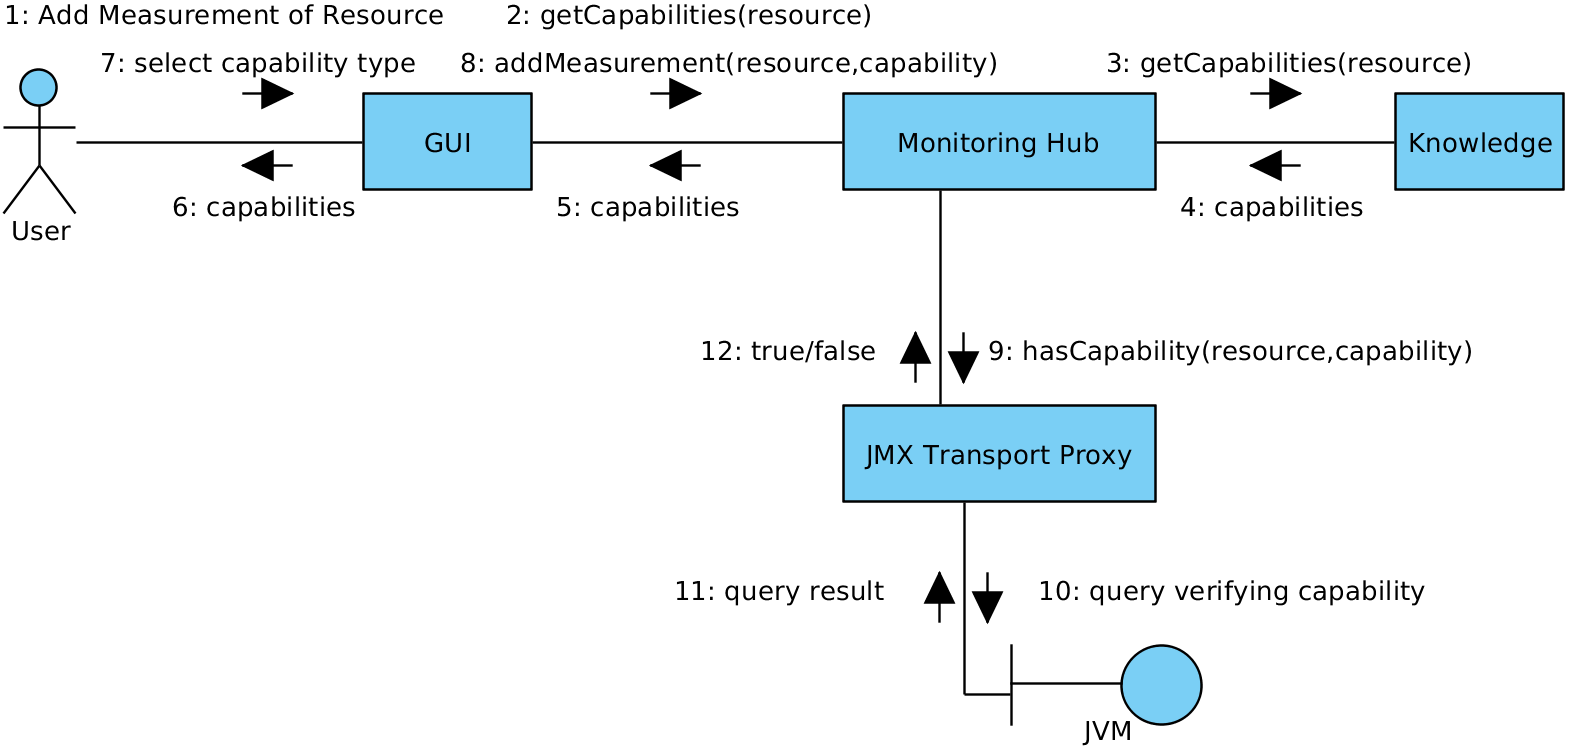
\includegraphics[width=0.9\textwidth]{comm_add_measurement}
  \caption{Communication diagram - adding of new measurement}
  \label{fig:comm_add_measurement}
\end{figure}

Addition of new measurement is a bit more straightforward than registration of new resources. All messages exchange
needed to achieve it can be found in Figure~\ref{fig:comm_add_measurement}. In this case, same as above, action is
initialized by a user. He or she chooses resource to add measurement of, and clicks appropriate button. In reaction
to this event, GUI  requests Monitoring Hub to get all possible capabilities that can be measured for resource type of
resource selected by the user. Monitoring Hub passes this request to Knowledge component. Then, results goes back GUI,
which can render appropriate user interface item, that will allow user to select which capability he or she would like
to measure. After selecting capability by user, GUI issues request to add new measurement to Monitoring Hub. The request
contains both resource identifier and ontology URL of capability. It verifies then, whether selected capability can be
measured with the selected resource. Such a validation is needed, because in certain circumstances it might
be impossible. To check this, Monitoring Hub sends verification request to transport proxy (JMX Transport Proxy in
example from Figure~\ref{fig:comm_add_measurement}). After successful verification, Monitoring Hub initializes scheduler
that will poll for capability values - measurement is successful created and started.


\begin{figure}[ht]
  \centering
  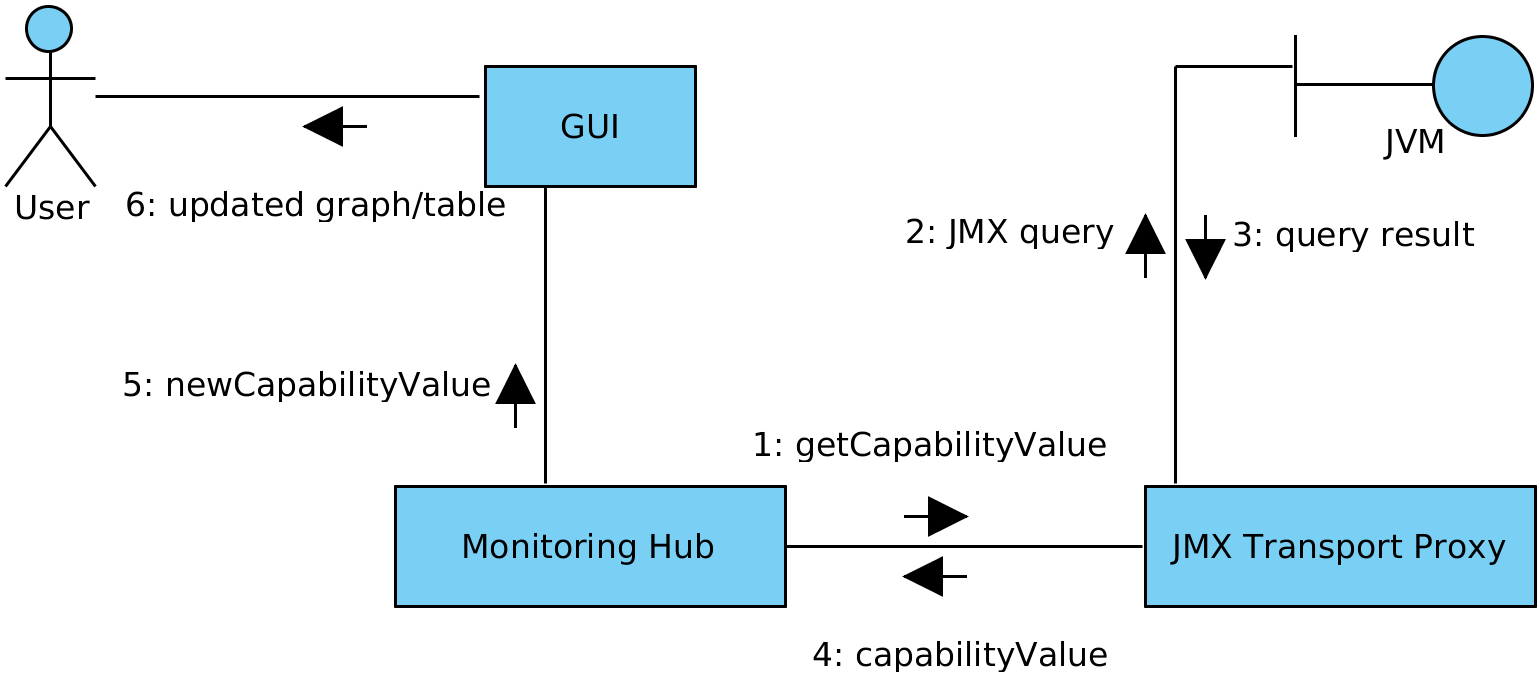
\includegraphics[width=0.7\textwidth]{comm_new_cap_value}
  \caption{Communication diagram - new capability value}
  \label{fig:comm_new_cap_value}
\end{figure}

Publishing new capability value is definitely most frequently used data flow in whole
system. Figure~\ref{fig:comm_new_cap_value} depicts this process. In contrast to previous communication diagrams, in
this case the Monitoring Hub component is initiator of this operation. Logic of this component manages
scheduled jobs responsible for polling of new capability value, and then pushing to listeners - previously registered
GUI components. In first step, Monitoring Hub calls appropriate (the one associated with resource in question) transport
proxy, which is JMX Transport Proxy in this case. JMX Transport Proxy maps generic getCapabilityValue request into
specific JMX query, sends the query to monitored JVM and returns result to Hub. Monitoring Hub uses this result to issue
notification dispatched through all registered listeners. GUI component, receives event and updates visualization graph,
which is being watched by a user.


\subsection{Communication protocol}
\label{subsec:arch_comm_protocol}
Communication protocol between components must allow both types of interactions: local and remote. By local interaction
I mean situation where all components constitutes single process and share same memory space. Remote system must use
remote interaction, when one or more components works as a separate process to other which enforce usage of network
stack for messages exchange. To make it possible, all communications will be performed using predefined, plain
interfaces, which aren't aware of underlying communication type. Such an approach decouples communication schema
from networking protocol being employed.

As a general rule for all communications between components, Transfer Object (also known as Value Object) design
pattern will be used\cite{0131422464}. This allows decoupling content of message of any complexity from serialization
mechanisms used. Following tables lists all transfer objects used in system. Additionally reader may find there purpose
of each object. 

% Add vertical spacing
\renewcommand*\arraystretch{1.2}


\begin{table}[ht] % ======================== CapabilityValue =====================================
\begin{tabular}{| m{1,5cm} | m{2,5cm} | m{8,5cm} |}
   \hline 
   \cellcolor[gray]{0.9} Field Type & \cellcolor[gray]{0.9} Field Name & \cellcolor[gray]{0.9} Details \\
   \hline 
   Number & numberValue & Numeric value of capability (optional, must be set if ValueType is number) \\
   Number[] & arrayValue & Vector value of capability (optional, must be set if ValueType is vector)  \\
   ValueType & valueType & Type of capability value - either numeric or vector\\
   Date & gatherTimestamp & Timestamp in UTF, when capability value have been gathered \\
   String & metricsId & Id of measurement to which this capability value belongs \\
   \hline 
\end{tabular}
 \caption{List of members of CapabilityValue Transfer Object}
 \label{tab:TO_CapValue}
\end{table} % ======================== CapabilityValue =====================================

Table~\ref{tab:TO_CapValue} contains list of members of CapabilityValue transfer object. This
object is used to notify listeners (GUI) about new capability value, and acts mostly as container for value, with
additional metadata. Most significant additional property that each CapabilityValue has is gatherTimestamp which points
to exact moment of time, when this capability value has been gathered. Using this property, system can use
CapabilityValue transfer objects, without worrying about implication of processing time on measurements presentation.

Members of MeasurementDefinition message format can be found in Table~\ref{tab:TO_MeasurementDef}. This object is used
by GUI component to define measurement that should be created during createMeasurement request.



\begin{table}[ht] % ======================== MeasurementDefinition =====================================
\begin{tabular}{| m{1,5cm} | m{2,5cm} | m{8,5cm} |}
   \hline 
   \cellcolor[gray]{0.9} Field Type & \cellcolor[gray]{0.9} Field Name & \cellcolor[gray]{0.9} Details \\
   \hline 
   String  & resourceUri &  Uri of resource that is covered by this measurement \\
   String & capabilityUri & Uri of capability that is covered by this measurement \\
   long & updateInterval & Interval in milliseconds defining how frequently value of measurement will be polled \\
   String & id & Identifier of this measurement \\ 
   \hline 
\end{tabular}
 \caption{List of members of MeasurementDefinition Transfer Object}
 \label{tab:TO_MeasurementDef}
\end{table} % ======================== MeasurementDefinition =====================================

Following tables:~\ref{tab:TO_Resource} and \ref{tab:TO_ResourceEvent} contains transfer objects needed by resources
management. Resource transfer object contains complete description of resource managed by system, additionally
MonitoringHub uses ResourceEvent to notify all listeners (GUI mostly) about resource's life cycle events.  

\begin{table}[ht] % ======================== Resource =====================================
\begin{tabular}{| m{1,5cm} | m{2,5cm} | m{8,5cm} | }
   \hline 
   \cellcolor[gray]{0.9} Field Type & \cellcolor[gray]{0.9} Field Name & \cellcolor[gray]{0.9} Details \\
   \hline
   String & typeUri & URI of resource's type according to currently used ontology \\
   String & uri & URI of resource in current resources tree hierarchy \\
   Map & properties & Static properties of resource (e.g. OS version) \\
   \hline 
\end{tabular}
 \caption{List of members of Resource Transfer Object}
 \label{tab:TO_Resource}
\end{table} % ======================== Resource =====================================



\begin{table}[ht] % ======================== ResourceEvent =====================================
\begin{tabular}{| m{1,5cm} | m{2,5cm} | m{8,5cm} | }
   \hline 
   \cellcolor[gray]{0.9} Field Type & \cellcolor[gray]{0.9} Field Name & \cellcolor[gray]{0.9} Details \\
   \hline
   Type & eventType & Enumeration that defines whether resources in this event have been added  or removed  \\
   List & resources & Collections of resources covered by this event \\
   \hline 
\end{tabular}
 \caption{List of members of ResourceEvent Transfer Object}
 \label{tab:TO_ResourceEvent}
\end{table} % ======================== ResourceEvent =====================================


% Remove vertical spacing
\renewcommand*\arraystretch{1}

%---------------------------------------------------------------------------
% Monitoring Hub component.
%
%---------------------------------------------------------------------------
\section{Monitoring Hub}
\label{sec:arch_monitoring_hub}

Monitoring Hub is the core component of the system. If using layered model to analyze application, Monitoring Hub should be treated as logic layer - placed between the presentation layer (GUI) and data access layer (transport proxies). It provides services to GUI and it uses Transport Proxy implementations and Knowledge component. Its main responsibilities include resources management (registering new resources, discovery dependent resources), measurements management (creation, pausing, resuming and termination) and creation of scheduled jobs that pools for capability values and pushes new values to registered listeners.

When user wants to start monitoring new resource, He or She must choose which Monitoring Hub to use. This decision, creates direct association between the chosen hub, the resource to monitor and all its child resources discovered during registration. This association defines that Monitoring Hub associated during registration and discovery process will process all further request calls related to given resource.

To make high-level components loosely coupled, Monitoring Hub is not aware of details about other components. To be able to provide its services it uses transport proxies and knowledge components, but it interacts with them only using commonly known interfaces. Additionally it is not aware about the existence of GUI component at all. It just provide services by implementing given interface, and it uses also common listener interfaces to notify about a variety of events.


\subsection{Decomposition of Monitoring Hub}

\begin{figure}[ht]
\centering
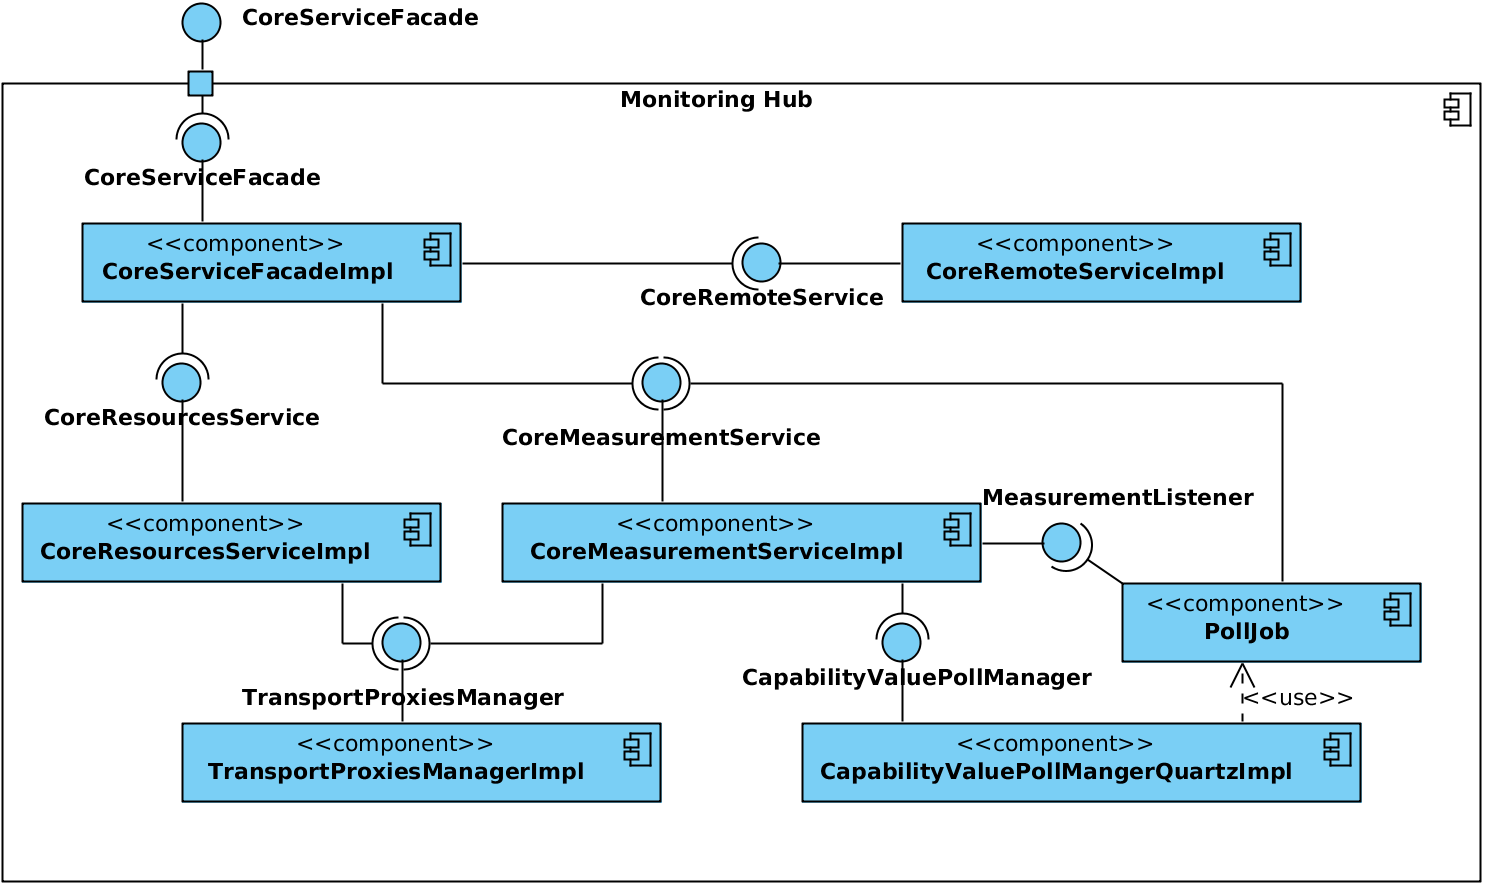
\includegraphics[width=0.9\textwidth]{decomposition_mon_hub}
\caption{Communication diagram - adding of new resource}
\label{fig:decomposition_mon_hub}
\end{figure}

Further decomposition of Monitoring Hub can be found in Figure~\ref{fig:decomposition_mon_hub}. This module is composed of following low level components:

\begin{itemize}

\item {\bf CoreServiceFacadeImpl}~~~~~~~~~~~~~~~~~~~~~~~~~~~~~~~~~~~~~~~~~~~~~~~~~~~~~~~~\linebreak
CoreServiceFacadeImpl is a facade that allows access to all Monitoring Hub functionalities from a single interface (CoreServiceFacade, shared with GUI and Monitoring Hub Application high level components). This wrapper eases remote access by exposing and using one interface with any remoting middle ware is easier than multiple ones. Having multiple interfaces in most cases would require multiple socket connections which can be a source of additional problems. We should tend to use as small amount connections as possible, because more connections system uses, than it becomes more and more prone to network configuration issues (e.g. firewalls). Additionally, using single facade improves code style, as with facade, only one interface has to be visible for all other components that are its clients.

\item {\bf CoreRemoteServiceImpl}~~~~~~~~~~~~~~~~~~~~~~~~~~~~~~~~~~~~~~~~~~~~~~~~~~~~~~~~\linebreak
CoreRemoteServiceImpl is a service responsible for processing requests related to remote management of Monitoring Hub. It has two main responsibilities: it allows registering remote listening interfaces and it dispatches local events (new resource, new capability value etc.) to remote listeners in aggregated manner. Distributed dispatch of events requires a bit different approach than a local one (local one, means dispatch inside of single JVM process). First of all, in most cases remote interface that will receive notifications with different signature, to allow handling exceptions related to networking. Additionally, to reduce the amount of remote calls and thus improve efficiency, CoreRemoteServiceImpl aggregates events into batches and notifies remote listeners using a generated package of them. Such an approach does not pollute measuring results, because each measurement value has associated gather timestamp (see~\ref{subsec:arch_comm_protocol}), initialized by component that grabs given value, at the exact moment, of measurement. Additionally, as events related to resources addition/removal don\rq{}t require such a strict time association, those events can be aggregated without any issues.

\item {\bf CoreResourcesServiceImpl}~~~~~~~~~~~~~~~~~~~~~~~~~~~~~~~~~~~~~~~~~~~~~~~~~~~~~~~~\linebreak
CoreResourcesServiceImpl is responsible for resources management: registering new ones, discovery of their children, returning all registered and discovered ones. It is also used to get more details about a resource, like capabilities that given resource may have.

\item {\bf CoreMeasurementServiceImpl}~~~~~~~~~~~~~~~~~~~~~~~~~~~~~~~~~~~~~~~~~~~~~~~~~~~~~~~~\linebreak
The CoreMeasurementServiceImpl can be used to create, pause, stop or terminate a measurement. Additionally it gathers current values of capabilities. It is used by the PollJob component for that purpose. It implements the MeasurementListener interface to be able to receive notifications about new capability values polled by the PollJob. 

\item {\bf TransportProxiesManagerImpl}~~~~~~~~~~~~~~~~~~~~~~~~~~~~~~~~~~~~~~~~~~~~~~~~~~~~~~~~\linebreak
The TransportProxiesManagerImpl component manages registered transport proxies. It is used by other components to get all transport proxies or to lookup a transport proxy that can be used to manage given resource.

\item {\bf CapabilityValuePollManagerImpl}~~~~~~~~~~~~~~~~~~~~~~~~~~~~~~~~~~~~~~~~~~~~~~~~~~~~~~~~\linebreak
CapabilityValuePollManagerImpl is responsible for scheduling polling jobs that are needed to run measurement.

\item {\bf PollJob}~~~~~~~~~~~~~~~~~~~~~~~~~~~~~~~~~~~~~~~~~~~~~~~~~~~~~~~~\linebreak
PollJob gets triggered with a configured interval. It simply polls for current capability value and push it to listeners specified during a creation stage.

\end{itemize}

\pagebreak

\subsection{Most important data flows}

This section contains a description of most salient data flows inside Monitoring Hub component. It covers actions of adding new resources, adding new measurements and dispatching new capability value notification.

Figure~\ref{fig:comm_mh_add_res} depicts communication diagram of adding new resources. In this scenario, external GUI component initiates action - registerResource request is the first step send by GUI to CoreServiceFacadeImpl. Facade simply delegates this call to CoreResourcesServiceImpl, which will perform actual registration. In the next step, CoreResourcesServiceImpl tries to find proxy capable to communicate with given resource by calling TransportProxiesManagerImpl. What should be noticed here, Transport Proxy is an external component to Monitoring Hub. After successfully obtaining transport proxy, CoreResourcesServiceImpl performs call to register given resource. If this registration succeeds, the CoreResourcesServiceImpl uses external Knowledge component, to get all types of child resources. Using this list, service requests TransportProxy to discover all children of the registered resource. After successful discovery, notification containing resources is being dispatched to all listeners. This can be done either directly, when given Monitoring Hub is embedded into GUI or remotely, using CoreRemoteServiceImpl.

\begin{figure}[ht]
\centering
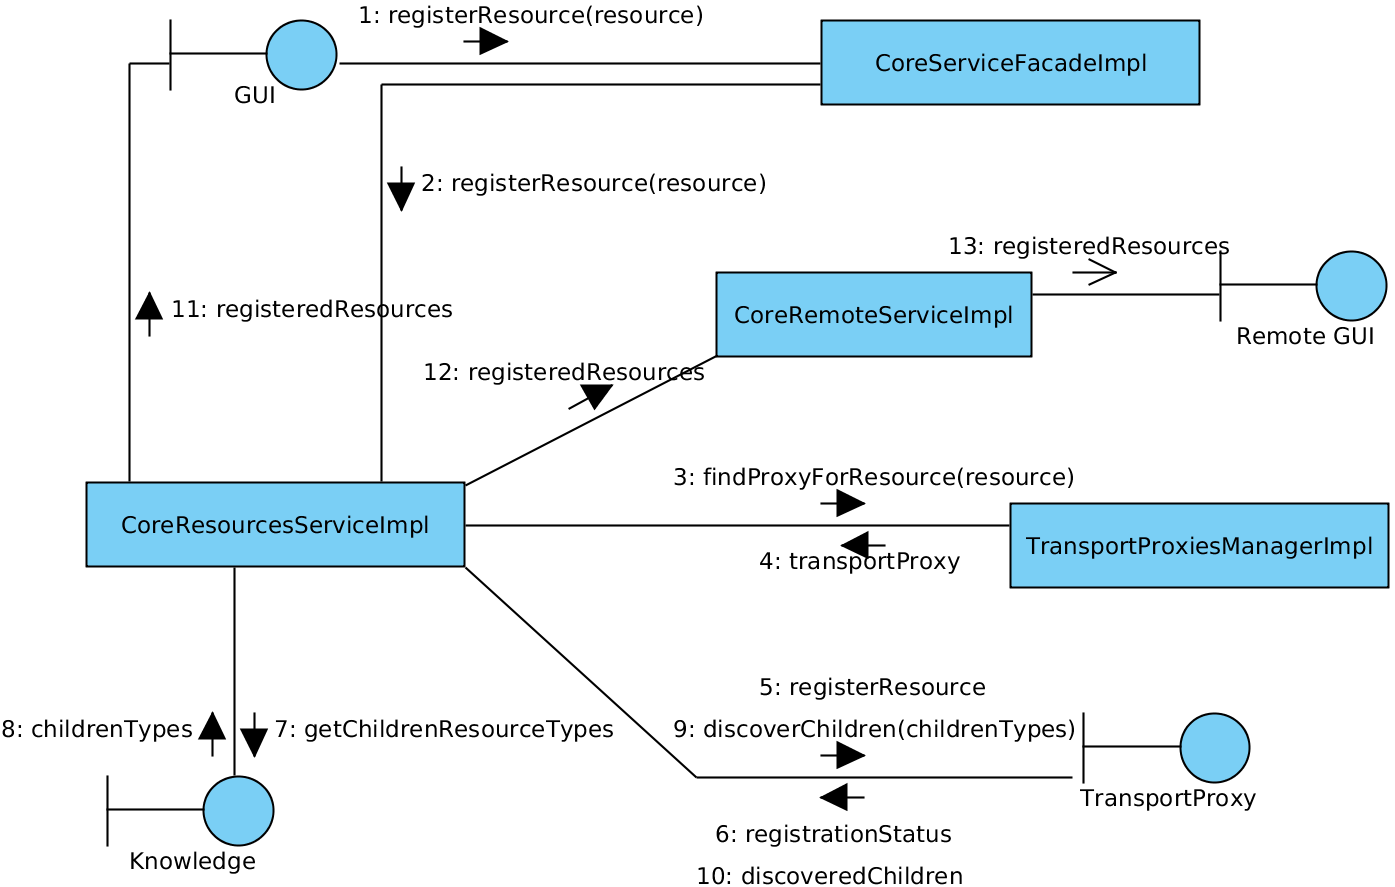
\includegraphics[width=0.9\textwidth]{comm_mh_add_res}
\caption{Monitoring Hub Communication diagram - adding new resource}
\label{fig:comm_mh_add_res}
\end{figure}

Communication diagram covering action of adding new measurements can be found in Figure~\ref{fig:comm_mh_add_measurement}. In this scenario, again GUI component is initiator. GUI component calls a getResourceCapabilities method, thus sends a first request to CoreServiceFacadeImpl. It will use those capabilities to show the user UI component, which will let user choose which capability should be measured. Facade delegates query to CoreResourcesServiceImpl, which passes it to external Knowledge component. Resulting list of capability URIs is being passed all way back, to the GUI component. Next, user selects, which capability should be measured. On selection event, GUI requests CoreServiceFacadeImpl to create measurement using given definition (see Table~\ref{tab:TO_MeasurementDef}). Request is delegated to CoreMeasurementServiceImpl which is responsible for the creation of measurement. Measurement service requests CapabilityValuePollManagerImpl to create a new instance of PollJob class. Measurement service, after creating polling job, generates measurement id, stores it internally with measurement definition, and returns it to requester. This identifier is then passed back to GUI, which will use it in any future call referring newly created measurement. Additionally it will be used to reference all incoming CapabilityValue objects.

\begin{figure}[ht]
\centering
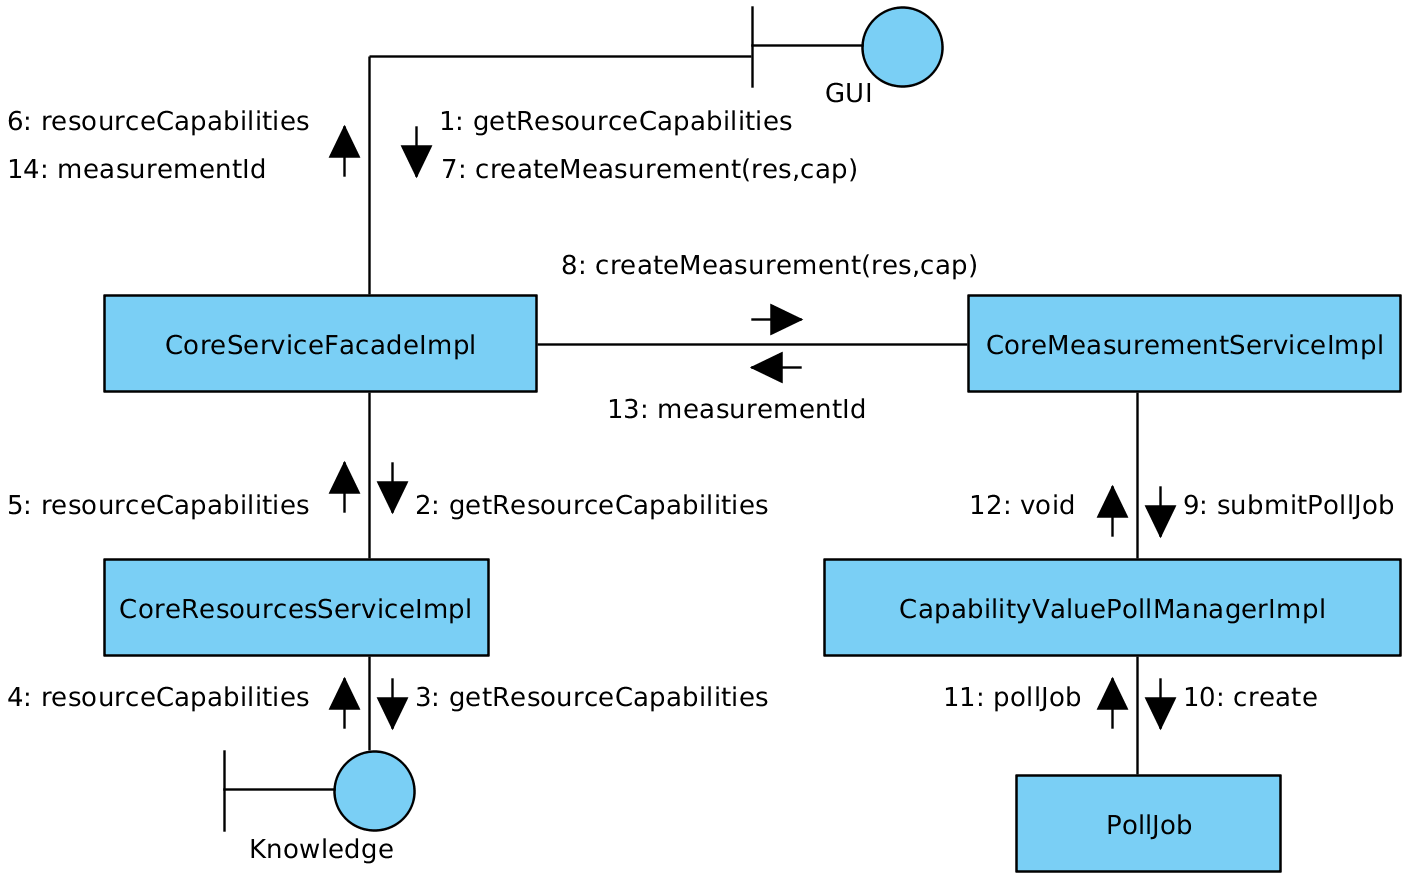
\includegraphics[width=0.8\textwidth]{comm_mh_add_measurement}
\caption{Monitoring Hub Communication diagram - adding new measurement}
\label{fig:comm_mh_add_measurement}
\end{figure}

Last data flow covered in this section describes gathering and publishing capability values. This time, CapabilityValuePollManagerImpl initiates the action. Its internal scheduler triggers previously created PollJob which contains measurement definition (URI's of resource and capability). Using those identifiers, PollJob calls CoreMeasurementServiceImpl to getCapabilityValue. Measurement service first looks up a transport proxy using TransportProxiesManagerImpl and then, using external TransportProxy, gets the capability value. In a subsequent step, gathered capability value is being pushed to all listeners, either directly (to listeners registered at CoreMeasurementServiceImpl) or using CoreRemoteServiceImpl to all remote listeners. What should be noticed here is that CoreRemoteServiceImpl notifies remote listeners in asynchronous and aggregated manner.

\begin{figure}[ht]
\centering
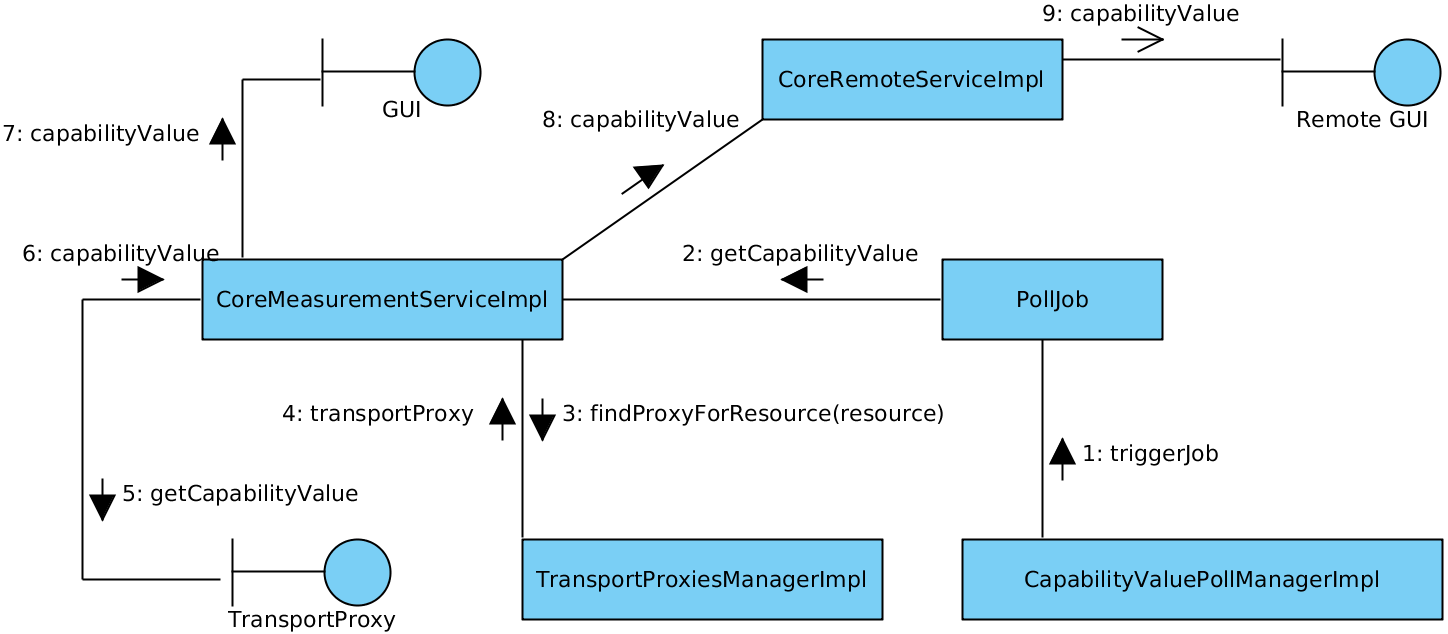
\includegraphics[width=1\textwidth]{comm_mh_new_cap_val}
\caption{Monitoring Hub Communication diagram - new capability value notification}
\label{fig:comm_new_cap_val}
\end{figure}
\pagebreak

%---------------------------------------------------------------------------
% Monitoring Hub application component.
%
%---------------------------------------------------------------------------
\section{Monitoring Hub Application}
\label{sec:arch_monitoring_hub_application}

Monitoring Hub Application is a component which has only one purpose that is crucial for using the system in a distributed manner - it allows using the Monitoring Hub remotely. A deeper analysis of the Monitoring Hub Application component will not be covered, because of its rather narrow functionality. It contains a code responsible for starting a process (a class with a \texttt{main} method), initializing the components of the Monitoring Hub and resolving dependencies between the components.

Additionally, in order to provide its distributed services, the Monitoring Hub Application module is responsible for the initialization of a remoting context. This involves a creation of all remote services and export of the Monitoring Hub functionality to remote clients using a ready to use RMI middleware.


%---------------------------------------------------------------------------
% Knowledge copmonent.
%
%---------------------------------------------------------------------------


\section{Knowledge component}
\label{sec:arch_knowledge}
 

Knowledge component is responsible for realization of semantic approach to proposed system. Although end-user can
barely notice its existence, it is crucial to allow high scalability and ease of use. Ontologies provided by
system gives generic measurement semantic. Such a approach allows user to get to know system only once and work using
it with many different types of hardware, protocols or more general - with any type of measured items that can be
mapped into generic components introduced by ontologies. Additionally it allows to work with all those different items
simultaneously, thus it makes possible monitoring application that are written using different technologies
and that are cooperating with each other.

\subsection{Default ontologies}

All system functionalities are built around two main ontologies - first one grouping resources, and the second, covering
resource capabilities. Main principle, I have been trying to follow, while designing them was to maximize wideness of
applications that can be monitored using SemSimMon system. User of application should be able to monitor wide range of
applications - from those running single process on one computing machine, up to highly distributed, grid-based ones.

To be able to describe proposed ontologies in more detail, two root concepts must be explained: concept of the
resource and the capability. Every other entity used in application is subclass of one of above. The resource
class wraps all components, either physical of virtual that are being used by user of application to
perform requested computations. Resource can be physical device that takes part in computation (hardware
resources), or any software component that can be either dependency (library) or is created by user (program, library).
On the other hand, the capability concept is used to generalize all measurable features of each resource. Capabilities
exists only in context of resources that contains them. Each resource may have multiple capabilities and given
capability may exist with multiple resources.

Above ontologies are being described using diagrams containing two types of relationships: is-a, and has-a. Is-a, is
formalized as rdfs:subClassOf and states that all the instances of one class are instances of
another\cite{rdfRef:2004}. Has-a relationship is used only to describe resources. It's main purpose is to show
composition arrangement, to ease understanding which resources are used by given parent resource to operate (e.g.
virtual machine uses class loader, garbage collector; computing node is built from one or more CPU, storage device,
network device and so on).

In following diagrams, entities are drawn as filled ellipse with entity name inside. The graphical representation of
is-a relationship between two entities is a hollow triangle shape on the supertype end of line that connects it to one
or more subtypes. To represent has-a relation, line with an arrowhead indicating entity owned by owner is used. This
notation is inspired by UML use case diagrams.

\pagebreak

\subsection{Resources ontology}
\label{subsec:arch_knowledge_resources}

Due to resources ontology complexity, diagrams containing both is-a and has-a relationships have been split into 3
parts: the one containing most general classes (application, node, cluster), second one for hardware resources
and software resources diagram.

\begin{figure}[ht]
  \centering
  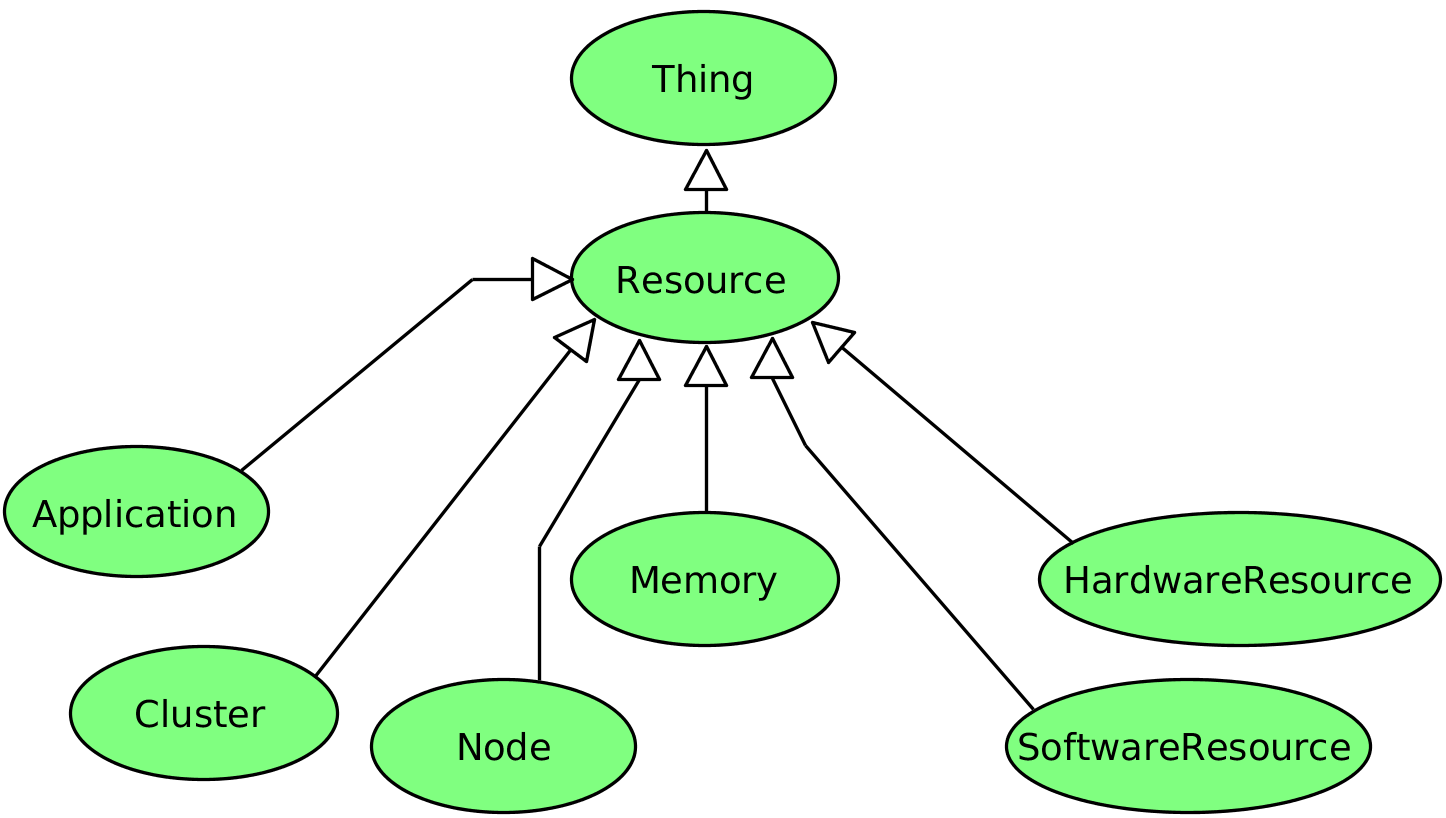
\includegraphics[width=0.6\textwidth]{onto_resources_admin}
  \caption{Diagram of is-a (rdfs:subClassOf) relationship between most general resource concepts}
  \label{fig:onto_resources_admin}
\end{figure}



Figure~\ref{fig:onto_resources_admin} depicts is-a relationship between general SemSimMon concepts. The root class of
every entity in OWL compliant ontologies is owl:Thing, as specified in OWL language reference\cite{owlRef:2004}. To
cover all possible resources - generic Resource class was introduced. It acts as a root concept for all other resources
and the only one direct subclass of owl:Thing. Resource has 6 direct subtypes: Application, Cluster, Node, Memory,
HardwareResource and SoftwareResource. Application and Cluster types are so called 'management' class resources - they
doesn't represent actual components, which can be used to perform computations. Instead, they can be used to aggregate
one or more elements, which allows user to building more manageable measurement structures. Application is most
important item, in context of has-a relationship, which illustrates Figure~\ref{fig:onto_resources_has_a_admin}. It
represent program created by user, which he or she wants to analyze using proposed tool. Each application, in
theoretical model may be running on multiple clusters, and multiple nodes.

Cluster refers to group of computing nodes which are connected using high efficiency network,thus in some way may be
treated as single entity. It is equivalent of site in OMIS nomenclature\cite{tl9702e}. Node can be interpreted as a
bridge between high-level resources and software, hardware resources. Generally speaking, it is smallest independent
computing unit, e.g. single PC or unit in a rack. It can be treated as administrative type of resource, as it's
not component that is used directly to aid computations, it rather aggregates such a components (all it's hardware with
operating system). But, on the other hand, node is an actual device that is used in processing. 

There exists also special class of resources - Memory. It's extracted to subclass Resource type directly, because there
exists at least two types of memory: software based (virtual memory) and hardware (physical memory) that share
common semantics.

\begin{figure}[ht]
  \centering
  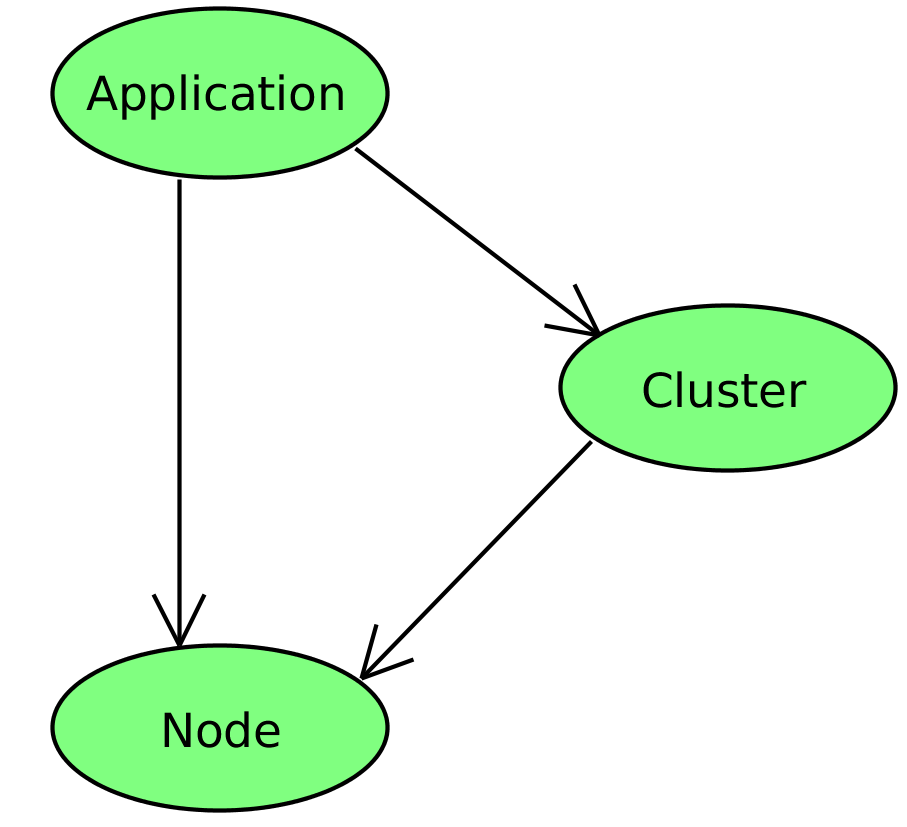
\includegraphics[width=0.3\textwidth]{onto_resources_has_a_admin}
  \caption{Diagram of has-a relationship between most general resource concepts}
  \label{fig:onto_resources_has_a_admin}
\end{figure}

\pagebreak


\begin{figure}[ht]
  \centering
  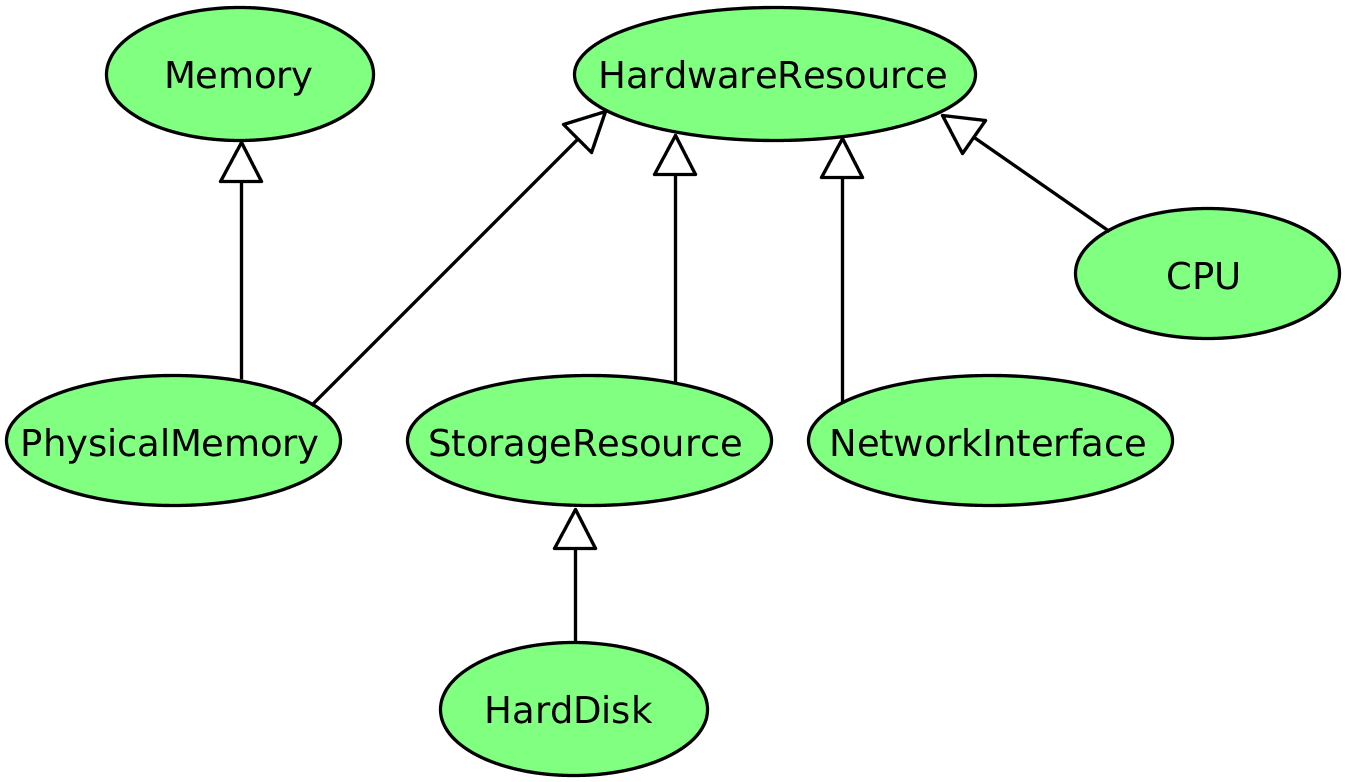
\includegraphics[width=0.6\textwidth]{onto_resources_hardware}
  \caption{Diagram of is-a relationship between hardware resources}
  \label{fig:onto_resources_hardware}
\end{figure}

Classes related to hardware resources, as can be seen in Figures~\ref{fig:onto_resources_hardware}
and~\ref{fig:onto_resources_has_a_hardware} were designed in a way that will allow to cover most of computer parts
available nowadays on market. Both diagrams are quite straightforward. HardwareResource has 4 direct sub-types:
PhysicalMemory, StorageResource, NetworkInterface and CPU. PhysicalMemory, is also subtype of Memory class, to share
common semantics, as was stated before. Also, StorageResource has one deriving class - HardDisk. 
Hardware resources has-a relationship diagram is even more elementary - Node may have all hardware resources, and there
are no other relations between those resources. Such a semantic allows to model any type of computing node - plain PC
with one, or more CPUs with at least one core (each core is treated as separate CPU).

\begin{figure}[ht]
  \centering
  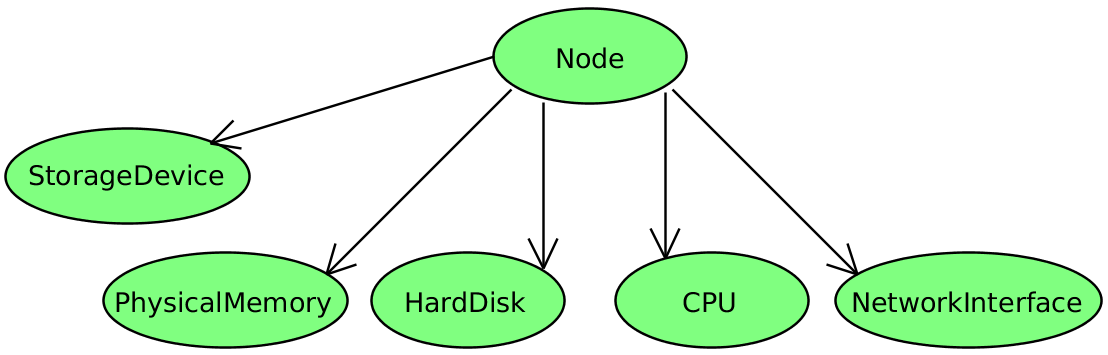
\includegraphics[width=0.7\textwidth]{onto_resources_has_a_hardware}
  \caption{Diagram of has-a relationship between hardware resources}
  \label{fig:onto_resources_has_a_hardware}
\end{figure}


\begin{figure}[ht]
  \centering
  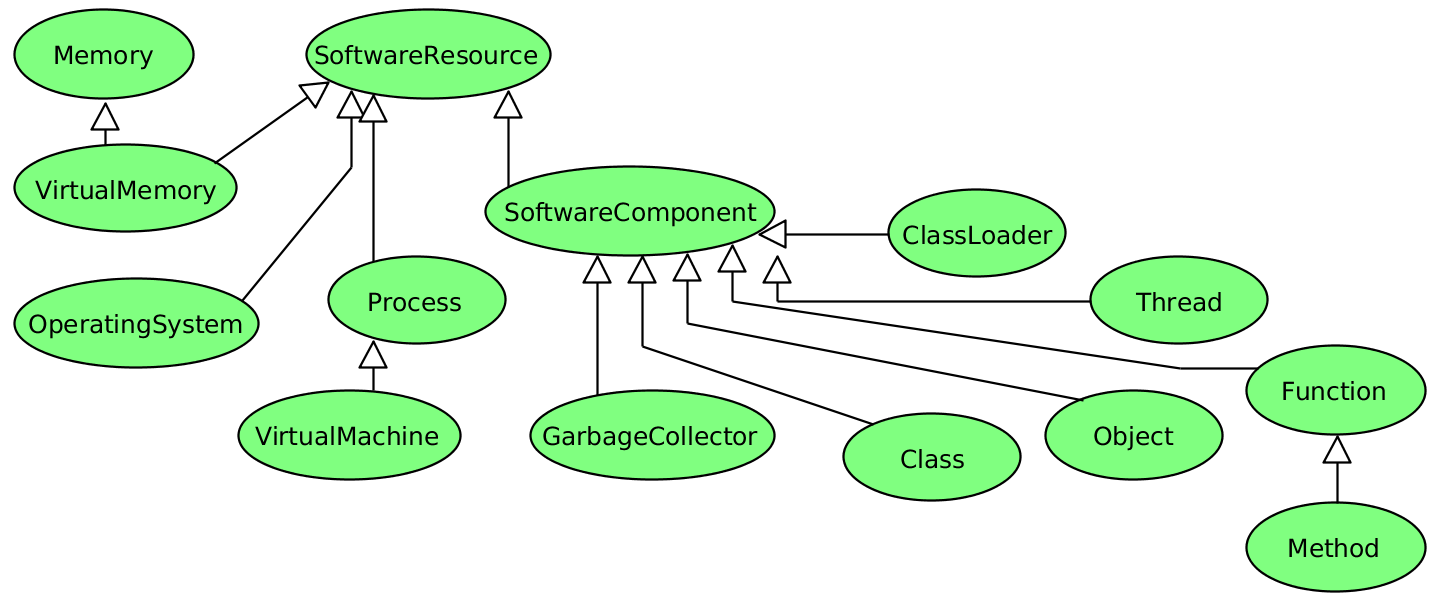
\includegraphics[width=0.9\textwidth]{onto_resources_software}
  \caption{Diagram of is-a relationship between software resources}
  \label{fig:onto_resources_software}
\end{figure}

System is aware of more software resource types then hardware ones. This implies more sophisticated relationships
between those concepts, which are depicted in Figures~\ref{fig:onto_resources_software} and
Figure~\ref{fig:onto_resources_has_a_software}. Class SoftwareResource has 4 direct subtypes: VirtualMemory (which
also derives from generic Memory concept), OperatingSystem, Process and SoftwareComponent concept. First 3 types are
quite straightforward and represent what one expects them to.
What should be noticed is special subtype of Process, namely VirtualMachine. It was extracted from more
general type, because of it's specific nature which differs it from all general purpose processes. Each virtual
machine acts as runtime environment for running application, thus it has specific features common for all virtual
machines, but unlikely seen in casual process.
SoftwareComponent resource type is logical wrapper for all low level software components that can be used to create
program. There are generic components, like Thread, Function. There are also types specific to Object Oriented
Programming: Class, Object, Method (which subtypes Function). The third group of SoftwareComponents subtypes is specific
to virtual machines. It contains only two items: GarbageCollector and ClassLoader.

Regarding ownership relations in software category there is one root concept - Node. Each node have: OperatingSystem,
and multiple Processes. Some processes may be VirtualMachines, thus this resource is last type that Node may own.
Each process may have following software components: Thread, Object, Class and Function. VirtualMachine may have
all components that generic process has, and also, two specific: ClassLoader and GarbageCollector. Additionally, Class
type owns one type of resource: Method. 
OperatingSystem resource may have only one resource type, namely VirtualMemory.


\begin{figure}[ht]
  \centering
  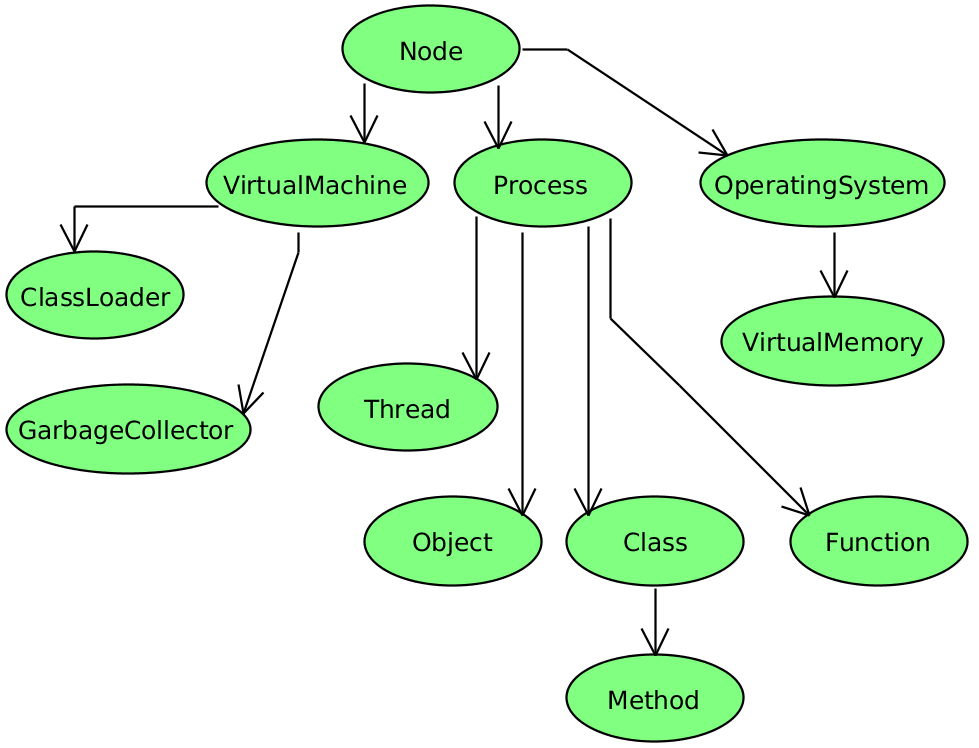
\includegraphics[width=0.7\textwidth]{onto_resources_has_a_software}
  \caption{Diagram of has-a relationship between software resources}
  \label{fig:onto_resources_has_a_software}
\end{figure}

\pagebreak

\subsection{Capabilities ontology}
\label{subsec:arch_knowledge_capabilitie}

For concepts related to capabilities of resources, only is-a relationships exists, which can be seen in
Figure~\ref{fig:onto_capabilities}. Because capability types are tightly coupled with resources, relations between them
reflects those between resources classes. 

There is one root concept, namely ResourceCapability, which subclasses rdf:Thing. It has 4 direct subtypes:
HardwareCapability, MemoryCapability, NodeCapability and SoftwareCapability. For hardware capability, there are only 2
deriving classes StorageCapability and CpuCapability. Since concept of VirtualMemory and PhysicalMemory are semantically
close, there is no need to subclass generic MemoryCapability, thus this type doesn't have any subtypes. NodeCapability
is another direct subtype of most generic ResourceCapability, which doesn't require any additional child types. 

Complex structure of software resources influences relationships between capabilities related to those components.
SoftwareCapability has 3 subtypes: OperatingSystemCapability, ProcessCapability and SoftwareComponentCapability.
Additionally, VirtualMachineCapability was extracted from ProcessCapability, because of same reasons that motivates
extraction of VirtualMachine resource type from Process - different semantics. The only one type that extends
SoftwareComponentCapability is ThreadCapability.


\begin{figure}[ht]
  \centering
  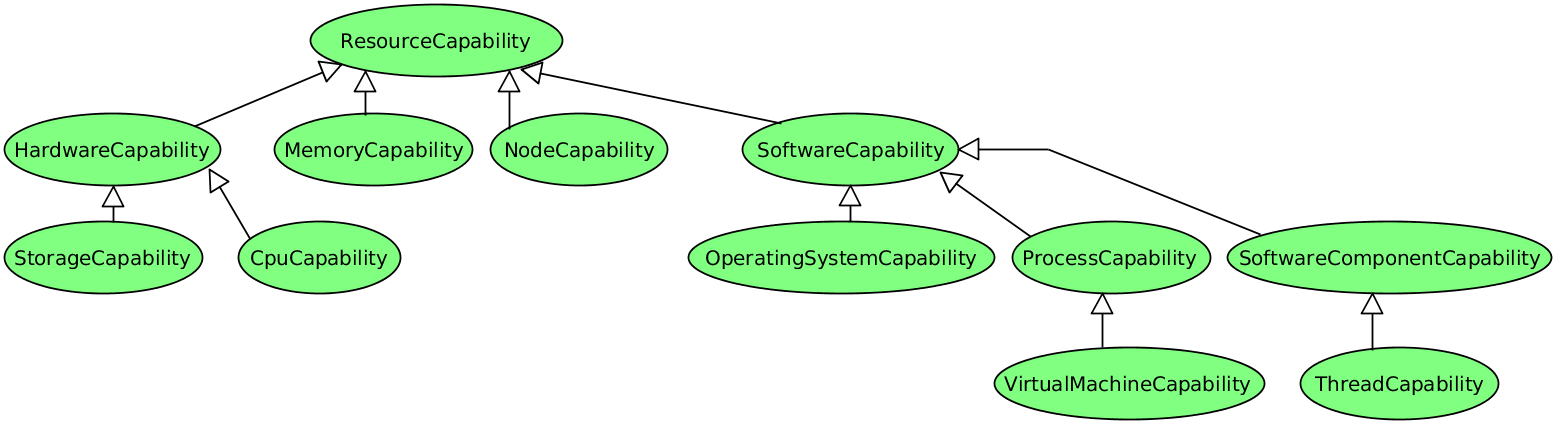
\includegraphics[width=1.0\textwidth]{onto_capabilities}
  \caption{Diagram of is-a relationship between capabilities}
  \label{fig:onto_capabilities}
\end{figure}






 
%---------------------------------------------------------------------------
% Transport proxy copmonent + it's realisations.
%
%---------------------------------------------------------------------------


\section{Transport Proxy component}
\label{sec:arch_tproxy}
 
Transport proxies are components responsible for communicating with external components that performs actual, low-level
analysis of processing tree and measurements. Each proxy implementation can specialize generic, ontology base concept
into item specific to platform or measuring system. All transport proxies implementation are being used by Monitoring
Hub component, and distributed in form of library (Java JAR). 

Because all proxies has rather straight purpose, further decomposition of those components won't be provided. In
following subsection, author covers overall design principles of Two transport proxies provided with initial
implementation of SemSimMon system.

 
\subsection{JMX Transport Proxy}

Implementation of transport proxy component responsible for integration with Java JMX consist of one root component -
JmxTransportProxy, several DiscoveryAgent and CapabilityProbe components. JmxTransportProxy component implements
interface used by other high-level system modules and performs all operations, delegating requests to appropriate
probes or discovery agents.

DiscoveryAgents are responsible for fetching all subresources of given resource. Each agent can be interpreted as a
mapping between ontology based, generic concept and item specific to JVM domain. Additionally, agents are responsible
for gathering all static properties of all discovered components.

If DiscoveryAgent can be seen as mapping between resource and JMX-specific entity, then CapabilityProbe should be
interpreted as mapping between generic capability described by ontology language into JMX specific feature. The only
responsibility of CapabilityProbe is to fetch value of capability that it can measure and using given resource.

To fulfill it's duties, JmxTransportProxy component maintains maps of discovery agents and capability probes. In both
cases map associates ontology URL of given concept to explicit probe or agent. Additionally it is responsible for
setting up and maintaining connection to JVM.


\subsection{OCM-G Transport Proxy}

OCM-G Transport Proxy component integrates SemSimMon with distributed monitoring system compliant with OMIS interface
specification. This implementation will use OMIS java bindings developed under OCM-G project. Design of this component
is similar to JMX transport proxy - there will be one OcmgTransportProxy component, responsible for maintaining
connections, associations and several probes and discovery agents.



 
%---------------------------------------------------------------------------
% Gui component.
%
%---------------------------------------------------------------------------


\section{GUI component}
\label{sec:arch_gui}

Graphical user interfaces are most commonly used form of interaction with user in modern computing. Designing decent
user interface is especially important due to aim of this work - creation of application allowing measuring and
visualization of monitored processes. Although GUI component has rather limited role of giving user control over
application and allow to view results of the work it's in fact most complex component. Additionally any shortcoming in
GUI is relatively difficult to be hidden by user, and that makes UI/UX (User Interface/User Experience) engineering so
important.

During designing user interface I've been trying to follow few general principles. First of all, I wanted used
interface to be as transparent as possible. Users should focus on their tasks instead of application. Because of that,
interface shouldn't be bloated with unnecessary options and steps that users need to achieve their goals should be as
short as possible. Next equally important interface item are visualizations. Because visualizations are most important
functionality of application, they need special concern. User should be able to view charts with results with out
any interruptions blocking or any other UI components that might be disturbing. What is also important, GUI must be
coherent to free user from chaos of being spread across multiple windows, desktops. 

From business logic point of view, GUI component will extensively use MVC design pattern\cite{gamma1995}. Each form,
window or more complex section need to have it's own View, responsible for presentation, Controller that collects
user's events and updates view on user's actions or system events. Application will have shared model, which will be
access point for underlaying components.
 


\subsection{Interface Mockups}

In this section, will try to describe mockups of most important views. The first mockup depicted in
Figure~\ref{fig:mock_main} shows main application view. Left edge of application window contains vertical tab pane
controller that will allow user to easily switch views covering 3 most important application contexts - resources,
measurements and visualizations. Another benefit of such a approach is that application has loads of space for what
user actually needs. The second most important component of main view is menu bar placed on top. It allows user
to perform bulk operations (e.g. pause all measurements) regardless of view he or she is currently. 

All subsequent mockups covers context specific views that will be rendered in main view's central pane.



\begin{figure}[ht]
  \centering
  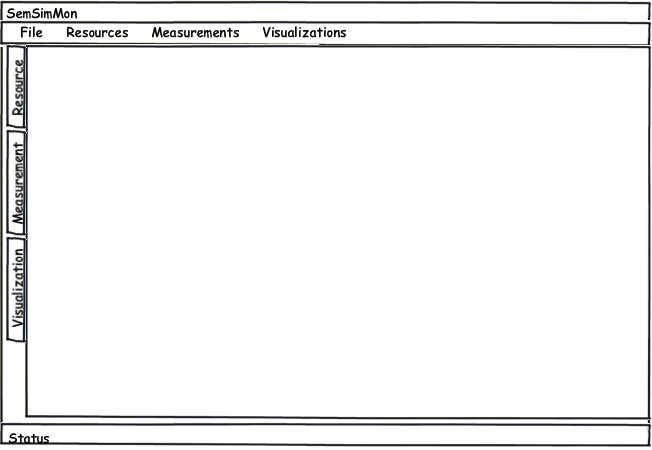
\includegraphics[width=0.7\textwidth]{mock_main}
  \caption{GUI application main view mockup}
  \label{fig:mock_main}
\end{figure}

When users starts to work with application He or She must add resources to be measured first. That's why resources view
is first, initial section shown to the user directly after page startup. Mockup of resources can bee seen in
Figure~\ref{fig:mock_resources}. The view is divided into 2 high level logical parts - the left pane covers global
resources context - users can browse measurement tree as well as add new resources into it. The right pane is specific
to resource selected by user and contains accordion with two sections. The upper one shows resource's static
attributes. The one below allow user to see snapshot of resource's dynamic state and check all of it's capabilities at
given point of time. To refresh those values, Refresh button was provided. Additionally, below accordion there are
several buttons allowing performing actions on given selected resource.

\begin{figure}[ht]
  \centering
  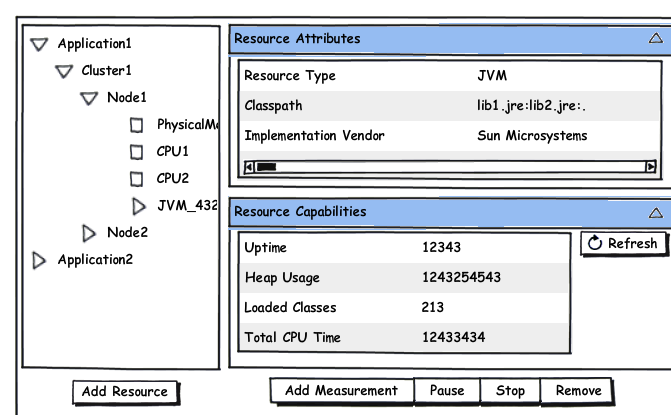
\includegraphics[width=0.7\textwidth]{mock_resources}
  \caption{GUI application resources pane}
  \label{fig:mock_resources}
\end{figure}

Next figure, Figure~\ref{fig:mock_measurements} covers measurements context of application. All measurements created
are listed on left side of this view. After selecting one accordion on right side shows details of selected
measurement. The upper section contain table with general informations. The lower one shows all measurement values
since the beginning. Additionally in this section user may copy the results into CSV format which can be easily
imported to spreadsheet application for further analysis. Using controls under measurements list, user can
pause, resume or remove measurement.

\begin{figure}[ht]
  \centering
  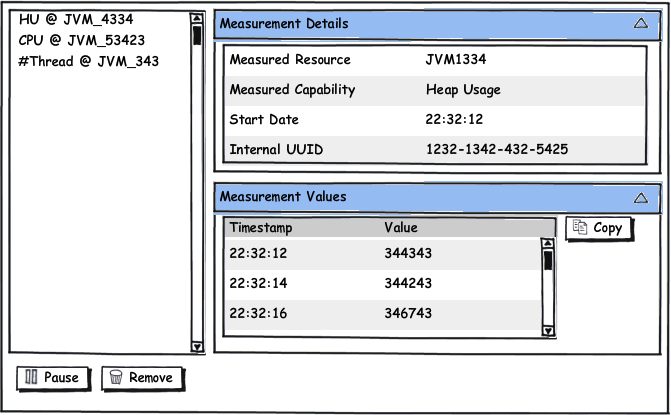
\includegraphics[width=0.7\textwidth]{mock_measurements}
  \caption{GUI application measurements pane}
  \label{fig:mock_measurements}
\end{figure}



\begin{figure}[ht]
  \centering
  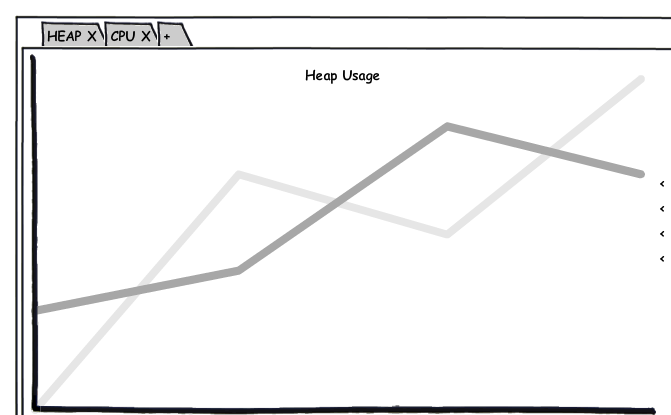
\includegraphics[width=0.7\textwidth]{mock_vis_clean}
  \caption{GUI application visualizations pane, clean view}
  \label{fig:mock_vis_clean}
\end{figure}

Appropriate visualizations display is probably most difficult for user experience engineering. During designing this UI
component I was inspiring myself from modest web browsers. The effects can be seen in Figure~\ref{fig:mock_vis_clean} -
in proposed solution every visualization is being rendered on separate, horizontal tab. To add new visualization, user
should just click last tab with appropriate icon. To remove visualization - user simply clicks cross icon on
visualization tab - just as He or She would close tab in browser. This gives visualization chart as much place as
application can give, and still allows user to easily control creation and disposal of visualization.

The biggest problem with such a approach is where to place controls of visualization. User must be able to choose which
measurements should be included in given visualization, as well as type of chart or other parameters. To address this
need, management pane was designed. It's hidden by default and is being displayed to the user, on mouse over right
edge of chart, marked with '<' signs. Layout of this pane is depicted in Figure~\ref{fig:mock_vis_options}. This
options pane contains form, divided into severals sections:

\begin{itemize}
 \item Visualization Options - user can here configure label of whole visualization, the one on tab pane
 \item Chart Options - allows setting chart's title (rendered on chart's graphics) and choose the chart type. User will
be able to use line (XY scatter), pie, bar and  spider web chart types.
 \item Measurements - gives control over which measurements should be included in given visualization. To add
measurement into visualization, user should click Add button and from displayed dialog choose which measurements should
be included. System doesn't give any constraints on measurements to be chosen, so it's up to the user to prepare
meaningful visualization. User will be able to remove given measurement from chart, by simply selecting it from list
and clicking Remove button.
 \item Actions - allows user to pause, resume visualization. Additionally user can copy to clipboard image containing
snapshot of visualization's chart.
\end{itemize}


\begin{figure}[ht]
  \centering
  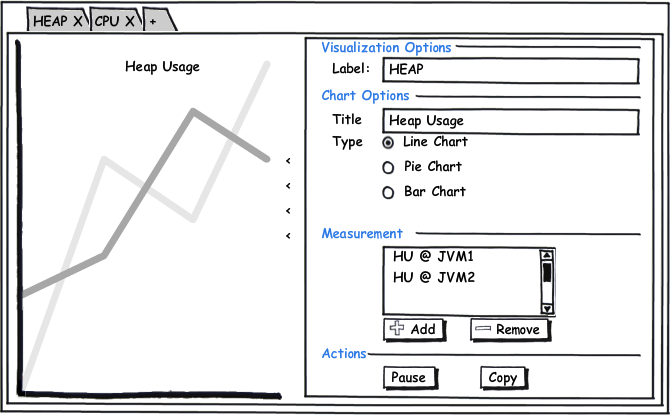
\includegraphics[width=0.7\textwidth]{mock_vis_options}
  \caption{GUI application visualizations pane, view with options pane}
  \label{fig:mock_vis_options}
\end{figure}



\subsection{Architecture}



